\documentclass{report}

\usepackage{tikz}
\usetikzlibrary{calc}
\usepackage{amssymb}

\begin{document}
	\begin{center}\begin{tikzpicture}
		\draw[blue] (2.75,-2) -- (2.75,3);
		\node[blue] at (3.2,3) (Komp) {$U^\perp$};
		
		\draw[thick] (0,0) -- (4,0);
		\draw[thick] (0,0) -- (1.5,1.5);
		\draw[thick] (4,0) -- (5.5,1.5);
		\draw[thick] (1.5,1.5) -- (5.5,1.5);
		\node at (3.5,0.4) (U) {$U$};
		\node at (0,2.5) (R) {$\mathbb{R}^3$};
		
		\coordinate (c2) at (2.75,0.75);
		\draw ($(c2) + (0:0.4)$) arc (0:90:0.4); % radius=4mm, initial=0, final=90
		\draw[thick] (2.90,0.90) circle (0.01);
	\end{tikzpicture}\end{center}

	\begin{center}\begin{tikzpicture}
		\draw[->] (-7,0) -- (-1,0);
		\draw[->] (-4,-3) -- (-4,3);
		\draw[thick] (-7,-1.5) -- (-1,1.5);
		\draw[fill=black] (-3,0.5) circle (0.05);
		\node at (-5,2) (real) {$\mathbb{R}^2$};
		\node at (-1,1.8) (gerade) {$L$};
		\node at (-1.7,0.5) (punkt) {$x=\left(\begin{array}{c}x_1 \\ x_2\end{array}\right)$};
		
		\draw[->] (1,0) -- (7,0);
		\draw[->] (4,-3) -- (4,3);
		\draw[thick] (2.5,3) -- (5.5,-3);
		\draw[fill=black] (4.5,-1) circle (0.05);
		\node at (5,2) (real) {$\left(\mathbb{R}^2\right)^*$};
		\node at (2.2,3) (annulator) {$L^0$};
		\node at (5.7,-1) (punkt2) {$a=(a_1,a_2)$};
	\end{tikzpicture}\end{center}

	\begin{center}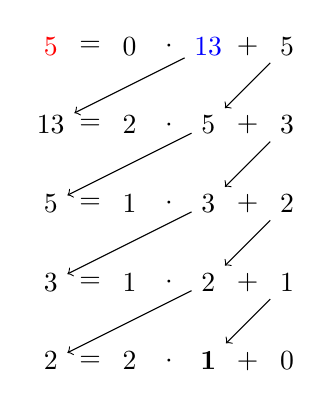
\begin{tikzpicture}
		\node at (0,0) (gleich) {$=$};
		\node at (0,-1) (gleich) {$=$};
		\node at (0,-2) (gleich) {$=$};
		\node at (0,-3) (gleich) {$=$};
		\node at (0,-4) (gleich) {$=$};
		
		\node at (1,0) (mal) {$\cdot$};
		\node at (1,-1) (mal) {$\cdot$};
		\node at (1,-2) (mal) {$\cdot$};
		\node at (1,-3) (mal) {$\cdot$};
		\node at (1,-4) (mal) {$\cdot$};
		
		\node at (2,0) (plus) {$+$};
		\node at (2,-1) (plus) {$+$};
		\node at (2,-2) (plus) {$+$};
		\node at (2,-3) (plus) {$+$};
		\node at (2,-4) (plus) {$+$};
		
		\node[red] at (-0.5,0) (erg1) {5};
		\node at (-0.5,-1) (erg2) {13};
		\node at (-0.5,-2) (erg3) {5};
		\node at (-0.5,-3) (erg4) {3};
		\node at (-0.5,-4) (erg5) {2};
		
		\node at (0.5,0) (fak1) {0};
		\node at (0.5,-1) (fak2) {2};
		\node at (0.5,-2) (fak3) {1};
		\node at (0.5,-3) (fak4) {1};
		\node at (0.5,-4) (fak5) {2};
		
		\node[blue] at (1.5,0) (quot1) {13};
		\node at (1.5,-1) (quot2) {5};
		\node at (1.5,-2) (quot3) {3};
		\node at (1.5,-3) (quot4) {2};
		\node at (1.5,-4) (quot5) {\textbf{1}};
		
		\node at (2.5,0) (plus1) {5};
		\node at (2.5,-1) (plus2) {3};
		\node at (2.5,-2) (plus3) {2};
		\node at (2.5,-3) (plus4) {1};
		\node at (2.5,-4) (plus5) {0};
		
		\draw[->] (quot1) -- (erg2);
		\draw[->] (quot2) -- (erg3);
		\draw[->] (quot3) -- (erg4);
		\draw[->] (quot4) -- (erg5);
		
		\draw[->] (plus1) -- (quot2);
		\draw[->] (plus2) -- (quot3);
		\draw[->] (plus3) -- (quot4);
		\draw[->] (plus4) -- (quot5);
	\end{tikzpicture}\end{center}
\end{document}